\documentclass{article}
\usepackage[margin=1in]{geometry}
\usepackage{amsmath, amsthm, amssymb}
\usepackage{physics}
\usepackage{float}
\usepackage{graphicx}
\usepackage{hyperref}
\usepackage{subcaption}


\theoremstyle{plain}
\newtheorem{proposition}{Proposition}

\theoremstyle{definition}
\newtheorem{definition}{Definition}

\theoremstyle{remark}
\theoremstyle{remark}


\title{Unstable Modes in Magnetic Nozzle}
\author{Hunt Feng}
\date{\today}

\begin{document}
\maketitle

\section{Equations of Motion}
\subsection{Linearized Equations of Motion}
The dynamics of magnetic nozzle can be characterized by conservation of mass and momentum,
\begin{align*}
    &\pdv{n}{t} + B\pdv{z}(\frac{nv}{B}) = 0\\
    &\pdv{v}{t} + v\pdv{v}{z} = -c_s^2\frac{1}{n}\pdv{n}{z}
\end{align*}
Usually, the magnetic field can be described by
\[ B(z) = B_0\left[ 1 + R\exp(-\frac{z^2}{\delta^2}) \right] \]
where $R$ and $\delta$ are some coefficients.

At equilibrium (stationary solution), we have $\pdv*{n_0}{t}=0$ and $\pdv*{v_0}{t}=0$, so $n_0$ and $v_0$ satisfy
\begin{align*}
    &\pdv{z}(\frac{n_0v_0}{B}) = 0 \\
    &v_0\pdv{v_0}{z} = -c_s^2\frac{1}{n_0}\pdv{n_0}{z} 
\end{align*}
Let $M\equiv v_0/c_s$, then it can be represented by Lambert function, 
\[ M = \left[ -W\left(-M_m^2 \frac{B(z)^2}{B_m^2}e^{-M_m^2}\right) \right]^{1/2} \]
where $B_m\equiv 1+R$ is the maximum magnetic field (or magnetic field at mid-point), and $M_m$ is the mach number at mid-point. Below shows a few cases of the solution.
\begin{itemize}
    \item $M_m < 1$, subsonic velocity profile.
    \item $M_m = 1$, accelerating or decelerating profile (depending on the branch of the Lambert function).
    \item $M_m > 1$, supersonic velocity profile
\end{itemize}
\begin{figure}[H]
    \centering
    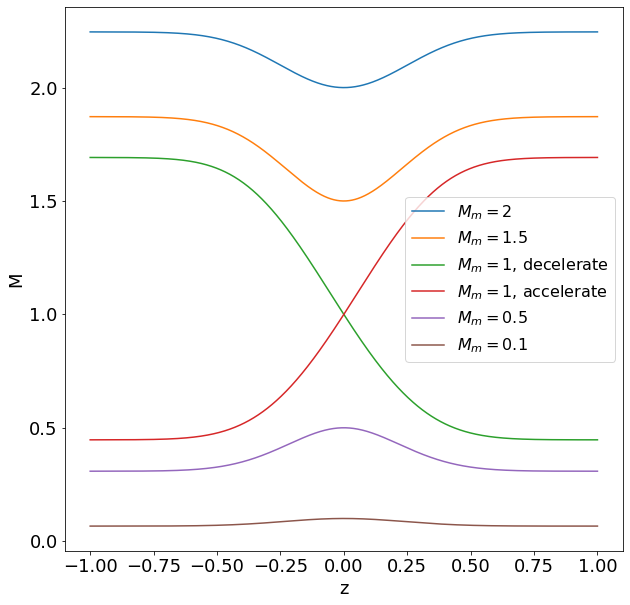
\includegraphics[width=0.7\linewidth]{img/nozzle-velocity-profile.png}
    \caption{$M_m < 1$, subsonic. $M_m = 1$, accelerating if we select Lambert function branch $k=0$ for $z<0$ and brach $k=-1$ for $z>=0$; decelerating if we choose branch $k=-1$ for $z<0$ and brach $k=0$ for $z>=0$. $M_m > 1$, supersonic.}
    \label{fig:nozzle-velocity-profile}
\end{figure}

For convenience, we nondimensionalize the equations by normalizing the velocity to $c_s$, $v\mapsto v/c_s$, $z$ to system length $L$, $z \mapsto z/L$ and time $t\mapsto c_s t/L$.
\begin{align}
    &\pdv{n}{t} + n\pdv{v}{z} + v\pdv{n}{z} - nv\frac{\partial_z B}{B} = 0 \\
    &n\pdv{v}{t} + nv\pdv{v}{z} = -\pdv{n}{z}
\end{align}
and the nondimensionalized equilibrium condition is
\begin{align}
    &\pdv{z}(\frac{n_0v_0}{B}) = 0 \label{eq:equilibrium-convervation-of-mass}\\
    &v_0\pdv{v_0}{z} = -\frac{1}{n_0}\pdv{n_0}{z} \label{eq:equilibrium-convervation-of-momentum}
\end{align}


\begin{proposition}
    Let $n = n_0(z) + \tilde{n}(z,t)$ and $v = v_0(z) + \tilde{v}(z,t)$, the linearized equations of motion are
    \begin{align}
        &\frac{1}{n_0}\pdv{\tilde{n}}{t} 
        + \pdv{\tilde{v}}{z} + v_0\tilde{Y} + \tilde{v}\frac{\partial_z n_0}{n_0} - \tilde{v}\frac{\partial_z B}{B} = 0 
        \label{eq:linearized-conservation-of-mass}
        \\
        &\pdv{\tilde{v}}{t} + \pdv{(v_0\tilde{v})}{z} = -\tilde{Y}
        \label{eq:linearized-conservation-of-momentum}
    \end{align}
    where 
    \[ \tilde{Y} \equiv \frac{1}{n_0}\pdv{\tilde{n}}{z} - \frac{\partial_z n_0}{n_0^2}\tilde{n} = \pdv{z}(\frac{\tilde{n}}{n_0}) \]
\end{proposition}
\begin{proof}
    We first derive Eq.(\ref{eq:linearized-conservation-of-mass}). We linearize Eq.(\ref{eq:equilibrium-convervation-of-mass}) by setting $n=n_0+\tilde{n}$ and $v=v_0+\tilde{v}$. By ignoring the second order perturbations, we obtain
    \begin{align*}
        &\pdv{(n_0+\tilde{n})}{t} 
        + (n_0+\tilde{n})\pdv{(v_0+\tilde{v})}{z} 
        + (v_0+\tilde{v})\pdv{(n_0+\tilde{n})}{z} 
        - (n_0+\tilde{n})(v_0+\tilde{v})\frac{\partial_z B}{B} = 0 \\
        \Rightarrow 
        &\pdv{\tilde{n}}{t} 
        + n_0\pdv{v_0}{z} + \tilde{n}\pdv{v_0}{z} + n_0\pdv{\tilde{v}}{z}
        + v_0\pdv{n_0}{z} + \tilde{v}\pdv{n_0}{z} + v_0\pdv{\tilde{n}}{z} 
        - (n_0v_0 + n_0\tilde{v} + \tilde{n}v_0)\frac{\partial_z B}{B} = 0 \\
        \Rightarrow
        &\frac{1}{n_0}\pdv{\tilde{n}}{t} 
        + \pdv{v_0}{z} + \frac{\tilde{n}}{n_0}\pdv{v_0}{z} + \pdv{\tilde{v}}{z}
        + \frac{v_0}{n_0}\pdv{n_0}{z} + \frac{\tilde{v}}{n_0}\pdv{n_0}{z} + \frac{v_0}{n_0}\pdv{\tilde{n}}{z} 
        - v_0\frac{\partial_z B}{B} - \tilde{v}\frac{\partial_z B}{B} - \tilde{n}\frac{v_0}{n_0}\frac{\partial_z B}{B} = 0
    \end{align*}
    Using the equilibrium condition Eq.(\ref{eq:equilibrium-convervation-of-mass}), some of the terms are canceled and the last term can be written as 
    \[ \tilde{n}\frac{v_0}{n_0}\frac{\partial_z B}{B} = \frac{\tilde{n}}{n_0}\left( \frac{\partial_z n_0}{n_0}v_0 + \pdv{v_0}{z} \right) \]
    Now, we are left with equation
    \[
        \frac{1}{n_0}\pdv{\tilde{n}}{t}
        + \pdv{\tilde{v}}{z}
        + v_0\underbrace{\left(\frac{1}{n_0}\pdv{\tilde{n}}{z} - \frac{\tilde{n}}{n_0}\frac{\partial_z n_0}{n_0}  \right)}_{\tilde{Y}}
        + \frac{\tilde{v}}{n_0}\pdv{n_0}{z}
        - \tilde{v}\frac{\partial_z B}{B} = 0
    \]

    To derive Eq.(\ref{eq:linearized-conservation-of-momentum}), we linearize the LHS of the conservation of momemtum
    \begin{align*}
        &(n_0+\tilde{n})\pdv{(v_0+\tilde{v})}{t} + (n_0+\tilde{n})(v_0+\tilde{v})\pdv{(v_0+\tilde{v})}{z} = -\pdv{n}{z} \\
        \Rightarrow 
        & \pdv{v_0}{t} + \frac{\tilde{n}}{n_0}\pdv{v_0}{t} + \pdv{\tilde{v}}{t} 
        + \left(v_0+\tilde{v}+\frac{\tilde{n}}{n_0}v_0\right)\pdv{(v_0+\tilde{v})}{z} = -\frac{1}{n_0}\pdv{n}{z}\\
        \Rightarrow
        & \pdv{v_0}{t} + v_0\pdv{v_0}{z} + \tilde{v}\pdv{v_0}{z} 
        = -\frac{1}{n_0}\pdv{n_0}{z} -\frac{1}{n_0}\pdv{\tilde{n}}{z} -v_0\frac{v_0}{z} - \frac{\tilde{n}}{n_0}v_0\pdv{v_0}{z} \\ 
    \end{align*}
    Using the equilibrium condition Eq.(\ref{eq:equilibrium-convervation-of-momentum}) on the RHS, we get the desired form.
\end{proof}

\section{Formulation of the problem}
\subsection{Polynomial Eigenvalue Problem}
\begin{proposition}
    \begin{equation}
        \pdv{z}\ln(\frac{n_0}{B}) = -\frac{1}{v_0}\pdv{v_0}{z}
        \label{eq:dv-ln}
    \end{equation}
\end{proposition}
\begin{proof}
    \[ \pdv{z}\ln(\frac{n_0}{B}) 
    = \frac{B}{n_0}\pdv{z}(\frac{n_0}{B})
    = \frac{1}{n_0}\frac{n_0}{z} + B\pdv{z}(\frac{1}{B})
    =
    \frac{1}{n_0}\frac{n_0}{z} \underbrace{- \frac{1}{n_0v_0}\pdv{n_0v_0}{z}}_{Eq.(\ref{eq:equilibrium-convervation-of-mass})}
    = -\frac{1}{v_0}\pdv{v_0}{z} \]
\end{proof}

\begin{proposition}
    Let $\tilde{n}\sim \exp(-i\omega t)$ and $\tilde{v} \sim \exp(-i\omega t)$, then we have the polynomial eigenvalue problem
    \begin{equation}
        \hspace{-0.5in}
            -\Omega^2 \tilde{v} 
            + 2\Omega\left(v_0\pdv{}{z} + \pdv{v_0}{z}\right) \tilde{v} 
            + \left[ (1-v_0^2)\pdv[2]{}{z} 
            -\left(3v_0 + \frac{1}{v_0}\right)\pdv{v_0}{z}\pdv{}{z} 
            - \left(1-\frac{1}{v_0^2}\right)\left(\pdv{v_0}{z}\right)^2 
            - \left(v_0+\frac{1}{v_0}\right)\pdv[2]{v_0}{z} \right]\tilde{v}
            = 0
            \label{eq:polynomial-eigenvalue-problem}
    \end{equation}
    where $\Omega\equiv i\omega$.
\end{proposition}
\begin{proof}
    \begin{align*}
        &\frac{1}{n_0}\pdv{\tilde{n}}{t} 
        + \pdv{\tilde{v}}{z} + v_0\tilde{Y} + \tilde{v}\frac{\partial_z n_0}{n_0} - \tilde{v}\frac{\partial_z B}{B} = 0 
        \\
        &\pdv{\tilde{v}}{t} + \pdv{(v_0\tilde{v})}{z} = -\tilde{Y}
    \end{align*}


    We plug Eq.(\ref{eq:linearized-conservation-of-momentum}) in to Eq.(\ref{eq:linearized-conservation-of-mass}), we have 
    \[ -i\omega\frac{\tilde{n}}{n_0} 
    + \pdv{\tilde{v}}{z} - v_0\left(-i\omega\tilde{v} + \pdv{(v_0\tilde{v})}{z}\right) + \tilde{v}\frac{\partial_z n_0}{n_0} - \tilde{v}\frac{\partial_z B}{B} = 0 \]

    Using the equilibrium condition Eq.(\ref{eq:equilibrium-convervation-of-mass}), we can eliminate the term $\partial_z B/B$,
    \begin{align*}
    &-i\omega\frac{\tilde{n}}{n_0} 
    + \pdv{\tilde{v}}{z} 
    + v_0\left(i\omega \tilde{v} - v_0\pdv{\tilde{v}}{z} - \tilde{v}\pdv{v_0}{z} \right)
    - \tilde{v}\frac{\partial_z v_0}{v_0} = 0\\
    \Rightarrow
    &-i\omega\frac{\tilde{n}}{n_0} 
    + i\omega v_0\tilde{v}
    + (1-v_0^2)\pdv{\tilde{v}}{z} 
    + \left(v_0+\frac{1}{v_0}\right)\pdv{v_0}{z}\tilde{v} = 0
    \end{align*}

    Now we take $\pdv*{t}$ on Eq.(\ref{eq:linearized-conservation-of-momentum}). Recall the fact that $\tilde{Y} = \pdv*{(\tilde{n}/n_0)}{z}$, we have
    \begin{align*}
        \omega^2\tilde{v} + i\omega\left(v_0\pdv{\tilde{v}}{z} + \tilde{v}\pdv{v_0}{z}\right) &= \pdv{t}\pdv{z}(\frac{\tilde{n}}{n_0}) \\
        \Rightarrow
        \omega^2\tilde{v} + i\omega\left(v_0\pdv{\tilde{v}}{z} + \tilde{v}\pdv{v_0}{z}\right) &= \pdv{z}(-i\omega v_0\tilde{v}
        - (1-v_0^2)\pdv{\tilde{v}}{z} 
        + \left(v_0+\frac{1}{v_0}\right)\pdv{v_0}{z}\tilde{v})
    \end{align*}
    Expand the RHS and collect terms, we get
    \begin{align*}
        &\omega^2 \tilde{v} \\ 
        &+2i\omega\left(v_0\pdv{}{z} + \pdv{v_0}{z}\right) \tilde{v} \\ 
        &+\left[ (1-v_0^2)\pdv[2]{}{z} 
        -\left(3v_0 + \frac{1}{v_0}\right)\pdv{v_0}{z}\pdv{}{z} 
        - \left(1-\frac{1}{v_0^2}\right)\left(\pdv{v_0}{z}\right)^2 
        - \left(v_0+\frac{1}{v_0}\right)\pdv[2]{v_0}{z} \right]\tilde{v}
        = 0
    \end{align*}
    Let $\Omega \equiv i\omega$, we obtain Eq.(\ref{eq:polynomial-eigenvalue-problem}).
\end{proof}

\subsection{Eigenvalue problem}
We can decouple the polynomial eigenvalue problem so that it becomes an eigenvalue problem.

Let $a=\Omega\tilde{v}$, then Eq.(\ref{eq:polynomial-eigenvalue-problem}) becomes

\begin{equation}
    \mqty[ O & I\\A_{21} & A_{22} ]\mqty[ \tilde{v}\\ a] = \Omega\mqty[ \tilde{v}\\ a]
    \label{eq:eigenvalue-problem}
\end{equation}
where $O$ is zero matrix, $I$ is identity matrix, and
\begin{align*}
    A_{21} &= 2\left(v_0\pdv{}{z} +\pdv{v_0}{z} \right) \\
    A_{22} &= (1-v_0^2)\pdv[2]{}{z} 
    -\left(3v_0 + \frac{1}{v_0}\right)\pdv{v_0}{z}\pdv{}{z} 
    - \left(1-\frac{1}{v_0^2}\right)\left(\pdv{v_0}{z}\right)^2 
    - \left(v_0+\frac{1}{v_0}\right)\pdv[2]{v_0}{z}
\end{align*}


\subsection{Variational Form}
\begin{definition}
    P and Q functions defined below can be used as an indicator of instabilities.
    \begin{itemize}
        \item P-function: 
        \begin{equation}
            P \equiv -\pdv{v_0}{z}\left(3v_0 + \frac{1}{v_0}\right)
            \label{eq:P-function}
        \end{equation}
        \item Q-function:
        \begin{equation}
            Q \equiv - \left(1-\frac{1}{v_0^2}\right)\left(\pdv{v_0}{z}\right)^2 
            - \left(v_0+\frac{1}{v_0}\right)\pdv[2]{v_0}{z}
            \label{eq:Q-function}
        \end{equation}
    \end{itemize}
\end{definition}

\begin{proposition}
    \begin{equation}
        (\omega_r^2-\gamma^2) \expval{\abs*{\tilde{v}}^2} 
        - 2\omega_r\expval{v_0 \Im\left(\tilde{v}^*\pdv{\tilde{v}}{z}\right)} 
        - \gamma\expval{\pdv{v_0}{z}\abs*{\tilde{v}}^2} 
        - \expval{(1-v_0^2)\abs{\pdv{\tilde{v}}{z}}^2 }
        + \expval{\left(Q-\frac{1}{2}\pdv{P}{z}\right)\abs*{\tilde{v}}^2} = 0
        \label{eq:stability-condition}
    \end{equation}

    This is the full instability condition, we can determine whether the motion is stable or not by examining the number of solutions $\gamma$. If there are two real solutions (two real $\gamma$), then it's unstable, otherwise it is stable.
\end{proposition}
\begin{proof}
    Starting from Eq.(\ref{eq:polynomial-eigenvalue-problem}), we multiply $\tilde{v}^*$ and take the average over the region, we have
\[ \omega^2 \expval{\abs*{\tilde{v}}^2} 
+ 2i\omega\left(\expval{v_0\tilde{v}^*\pdv{\tilde{v}}{z}} 
+ \expval{\pdv{v_0}{z}\abs*{\tilde{v}}^2}\right) 
+ \left[ \expval{(1-v_0^2)\tilde{v}^*\pdv[2]{\tilde{v}}{z} }
+ \expval{P\tilde{v}^*\pdv{\tilde{v}}{z} }
+ \expval{Q\abs*{\tilde{v}}^2} \right]
= 0  \]

Let $\omega \equiv \omega_r + i\gamma$, then
\[ (\omega_r^2-\gamma^2+2i\omega_r\gamma) \expval{\abs*{\tilde{v}}^2} 
+ 2(i\omega_r - \gamma)\left(\expval{v_0\tilde{v}^*\pdv{\tilde{v}}{z}} 
+ \expval{\pdv{v_0}{z}\abs*{\tilde{v}}^2}\right) 
+ \expval{(1-v_0^2)\tilde{v}^*\pdv[2]{\tilde{v}}{z} }
+ \expval{P\tilde{v}^*\pdv{\tilde{v}}{z} }
+ \expval{Q\abs*{\tilde{v}}^2}
= 0  \]

We split the equation into real and imaginary part.
\begin{itemize}
    \item Real: \\
    There are two useful simplifications to keep in mind,
    \begin{align*}
        &\Re\left(\tilde{v}^*\pdv{\tilde{v}}{z}\right) 
        = \frac{1}{2}\left(\tilde{v}^*\pdv{\tilde{v}}{z} + \tilde{v}\pdv{\tilde{v}^*}{z}\right) 
        = \frac{1}{2}\pdv{\abs{\tilde{v}}^2}{z} \\
        &\expval{\Re\left(\tilde{v}^*\pdv[2]{\tilde{v}}{z}\right) } 
        = \expval{\frac{1}{2}\left(\tilde{v}^*\pdv[2]{\tilde{v}}{z} + \tilde{v}\pdv[2]{\tilde{v}^*}{z}\right)}
        = \expval{\frac{1}{2}\left( \pdv{z}(\tilde{v}^*\pdv{\tilde{v}}{z}) + \pdv{z}(\tilde{v}\pdv{\tilde{v^*}}{z}) - 2\abs{\pdv{\tilde{v}}{z}}^2 \right)}
        = \expval{\abs{\pdv{\tilde{v}}{z}}^2}
    \end{align*}
    The second formula uses the fact $\tilde{v}=0$ on boundaries (Dirichlet condition), so $\expval{\pdv*{\text{product of }\tilde{v}}{z}} = 0$.

    Now we separate the real part,
    \begin{align*}
        (\omega_r^2-\gamma^2) \expval{\abs*{\tilde{v}}^2} 
        - 2\omega_r\expval{v_0 \Im\left(\tilde{v}^*\pdv{\tilde{v}}{z}\right)} 
        &- \gamma\expval{v_0 \pdv{\abs{\tilde{v}}^2}{z}} 
        - 2\gamma\expval{\pdv{v_0}{z}\abs{\tilde{v}}^2} \\
        &-\expval{(1-v_0^2) \abs{\pdv{\tilde{v}}{z}} }
        + \expval{\frac{1}{2}P\pdv{\abs{\tilde{v}}^2}{z}}
        + \expval{Q\abs*{\tilde{v}}^2} = 0
    \end{align*}

    The term with $\gamma$ can combine by swithing the position of $\pdv*{z}$,
    \[ - \gamma\expval{v_0 \pdv{\abs{\tilde{v}}^2}{z}} 
    - 2\gamma\expval{\pdv{v_0}{z}\abs{\tilde{v}}^2}
    = - \gamma\expval{\pdv{v_0}{z}\abs{\tilde{v}}^2} \]

    The $P$ and $Q$ term can combine as well
    \[ \expval{\frac{1}{2}P\pdv{\abs{\tilde{v}}^2}{z}}
    + \expval{Q\abs*{\tilde{v}}^2}
    = \expval{ \left(Q - \frac{1}{2}\pdv{P}{z}\right)\abs{\tilde{v}}^2 } \]

    The desired instability condition follows.

    \item Imaginary: \\ 
    Although the imaginary part is not important, we derive it too.

    This time, we notice that 
    \[ \expval{ \Im\left(\tilde{v}^*\pdv[2]{\tilde{v}}{z}\right) } 
    = \expval{\frac{1}{2}\left(\tilde{v}^*\pdv[2]{\tilde{v}}{z} - \tilde{v}\pdv[2]{\tilde{v}^*}{z}\right)}
    = \expval{\frac{1}{2}\left( \pdv{z}(\tilde{v}^*\pdv{\tilde{v}}{z}) - \pdv{z}(\tilde{v}\pdv{\tilde{v^*}}{z}) \right)}
    = 0 \]

    \[
        2\omega_r\gamma \expval{\abs*{\tilde{v}}^2} 
        + \omega_r\expval{v_0\pdv{\abs*{\tilde{v}}^2}{z}}
        + 2\omega_r\expval{\pdv{v_0}{z}\abs*{\tilde{v}}^2}
        - 2\gamma \expval{v_0\Im\left(\tilde{v}^*\pdv{\tilde{v}}{z}\right)}
        + \expval{P\Im\left(\tilde{v}^*\pdv{\tilde{v}}{z}\right)} = 0
    \]
\end{itemize}
\end{proof}

\begin{proposition}
    For oscillations where $\omega_r\to 0$, the instability condition becomes
    \[ -\gamma^2 \expval{\abs*{\tilde{v}}^2} 
    + \gamma\expval{\pdv{v_0}{z}\abs*{\tilde{v}}^2} 
    - \expval{(1-v_0^2)\abs{\pdv{\tilde{v}}{z}}^2 }
    + \expval{\left(Q-\frac{1}{2}\pdv{P}{z}\right)\abs*{\tilde{v}}^2} = 0 \]
    
    Therefore, unstable modes occur if 
    \[ \expval{\pdv{v_0}{z}\abs*{\tilde{v}}^2}^2 + 4\expval{\abs*{\tilde{v}}^2}\left( - \expval{(1-v_0^2)\abs{\pdv{\tilde{v}}{z}}^2 }
    + \expval{\left(Q-\frac{1}{2}\pdv{P}{z}\right)\abs*{\tilde{v}}^2} \right) > 0   \]
\end{proposition}


\newpage
\section{Numerical Experiments}
\subsection{Constant velocity profile}
If we set $v_0$ to Constant, then the eigenvalue 
\begin{equation}
    -\Omega^2 \tilde{v} 
    + 2\Omega v_0\pdv{}{z} \tilde{v} 
    + (1-v_0^2)\pdv[2]{}{z} \tilde{v}
    = 0
    \label{eq:constant-v-problem}
\end{equation}
where $\Omega\equiv i\omega$.

Then we have non-zero analytical solution 
\begin{equation}
    \tilde{v} = \exp(-\frac{\Omega}{v_0+1})\left[ \exp(\Omega\frac{z+1}{v_0+1}) - \exp(\Omega\frac{z+1}{v_0-1}) \right] \text{ where } \Omega=\frac{in\pi(1-v_0^2)}{2}
\end{equation}
Therefore, $\omega = -i\Omega = n\pi(1-v_0^2)/2$ are real. All modes are stable.
\begin{figure}[H]
    \centering
    \begin{subfigure}[b]{0.45\linewidth}
        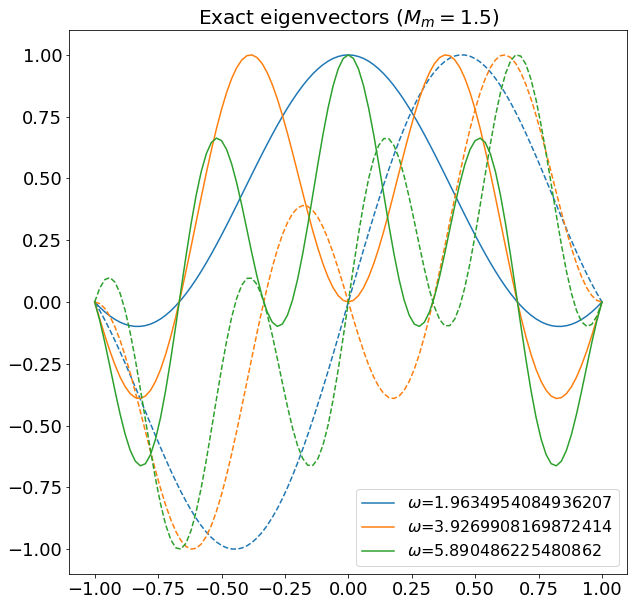
\includegraphics[width=\linewidth]{img/eigenfunctions-constant-v-exact.png}
        \caption{First few exact eigenfunctions(ground mode not included).}
    \end{subfigure}%
    \begin{subfigure}[b]{0.45\linewidth}
        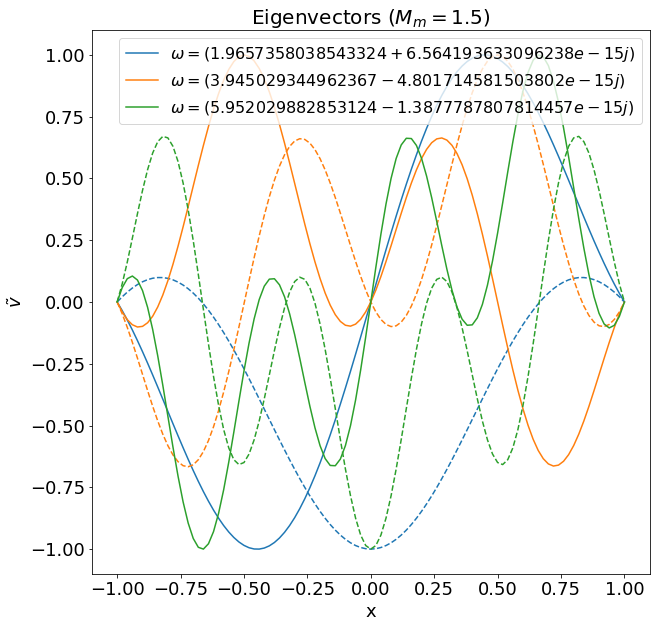
\includegraphics[width=\linewidth]{img/eigenfunctions-constant-v.png}
        \caption{First few numerical eigenfunctions by solving Eq.(\ref{eq:eigenvalue-problem}).}
    \end{subfigure}
    \caption{We see that the numerical eigenfunctions match the theoretical results. The numerical results are obtained by solving Eq.(\ref{eq:eigenvalue-problem}). Same conclusion can be drawn by solving Eq.(\ref{eq:polynomial-eigenvalue-problem}).}
    \label{fig:eigenvectors-constant-v}
\end{figure}

\subsubsection{"Unstable modes" for $v_0>1$}

\begin{figure}[H]
    \centering
    \begin{subfigure}[b]{0.5\linewidth}
        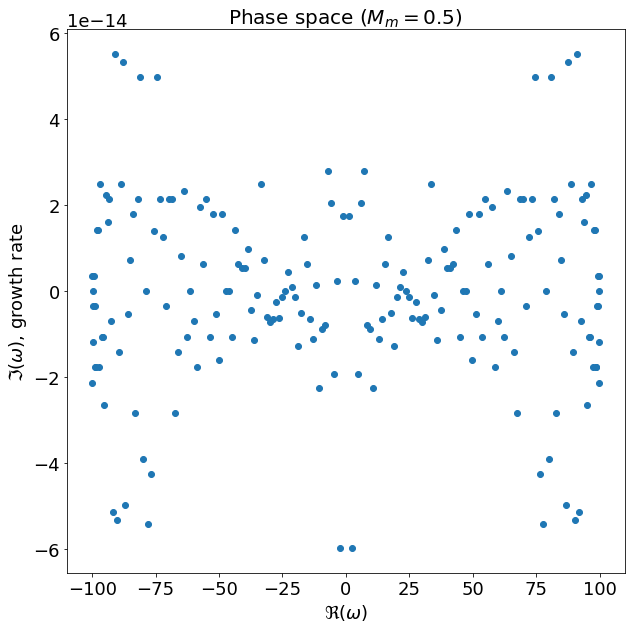
\includegraphics[width=\linewidth]{img/phase-space-constant-v<1.png}
        \caption{For $v_0<1$, all modes are stable.}
    \end{subfigure}%
    \begin{subfigure}[b]{0.5\linewidth}
        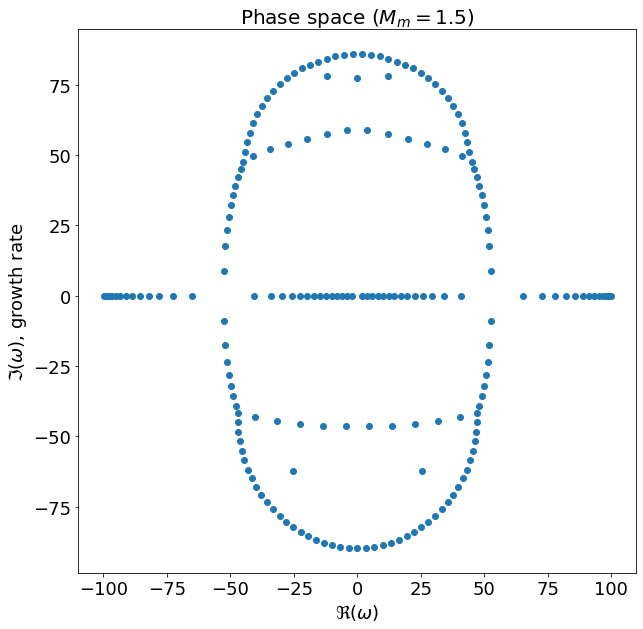
\includegraphics[width=\linewidth]{img/phase-space-constant-v>1.png}
        \caption{For $v_0>1$, it seems there are unstable modes.}
    \end{subfigure}
    \caption{It seems there are unstable modes for $v_0>1$.}
    \label{fig:phase-space-constant-v}
\end{figure}

If we plot the eigenfunctions for the "unstable modes", we see that
\begin{figure}[H]
    \centering
    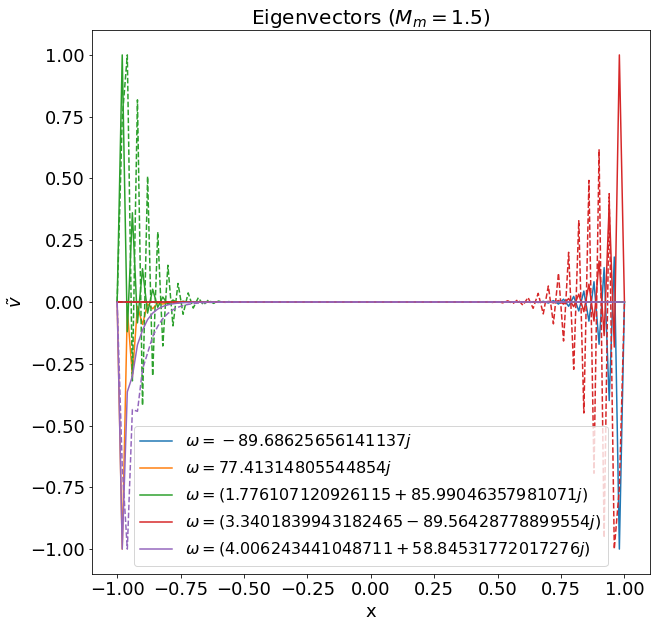
\includegraphics[width=0.5\linewidth]{img/eigenvectors-bad.png}
    \caption{The eigenfunctions do not look right. For both equally-spaced finite difference differentiation matrix and Chebyshev differentiation matrix, these eigenfunctions will occur.}
\end{figure}


\subsection{Subsonic case}
The stability condition Eq.(\ref{eq:stability-condition} is a quadratic equation about $\gamma$. Let 
\begin{align*}
    &a = -\expval{\abs*{\tilde{v}}^2} \\
    &b = -\expval{\pdv{v_0}{z}\abs*{\tilde{v}}^2} \\
    &c = \omega_r^2\expval{\abs*{\tilde{v}}^2} 
    - 2\omega_r\expval{v_0 \Im\left(\tilde{v}^*\pdv{\tilde{v}}{z}\right)} 
    - \expval{(1-v_0^2)\abs{\pdv{\tilde{v}}{z}}^2 }
    + \expval{\left(Q-\frac{1}{2}\pdv{P}{z}\right)\abs*{\tilde{v}}^2} = 0
\end{align*}
then the full instability condition becomes 
\[ D \equiv b^2 - 4ac \]

If the discriminant $D>0$, it is unstable. If $D<0$, it is stable. 

Subsonic modes are stable. The stability condition $D<0$. Moreover, the eigenvalues are real.


\begin{figure}[H]
    \centering
    \begin{subfigure}[b]{0.5\linewidth}
        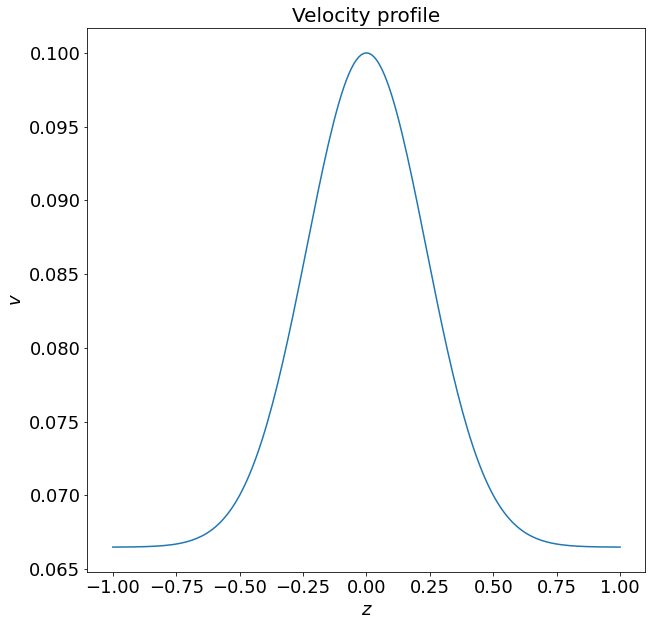
\includegraphics[width=\linewidth]{img/velocity-profile-subsonic.png}
        \caption{Subsonic velocity profile.}
    \end{subfigure}%
    \begin{subfigure}[b]{0.5\linewidth}
        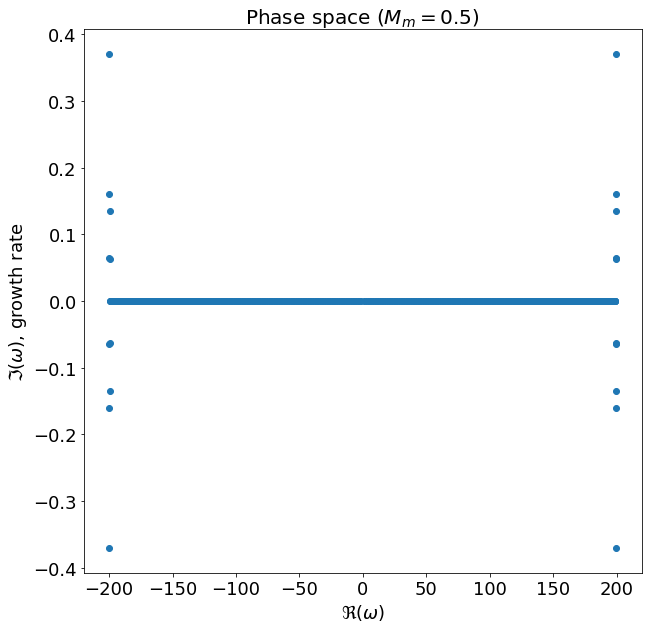
\includegraphics[width=\linewidth]{img/phase-space-subsonic.png}
        \caption{$\omega$'s are real, meaning that it is stable.}
    \end{subfigure}
    \caption{Solution to the polynomial eigenvalue problem Eq.(\ref{eq:polynomial-eigenvalue-problem}) with subsonic velocity profile. $\omega$'s are pure imaginary numbers, meaning that subsonic mode should be stable for most cases.}
    \label{fig:subsonic}
\end{figure}

\newpage
\subsection{Accelerating case}
Accelerating modes are unstable.

The stability condition for ground state is $D=0.00062>0$.

\begin{figure}[H]
    \centering
    \begin{subfigure}[b]{0.5\linewidth}
        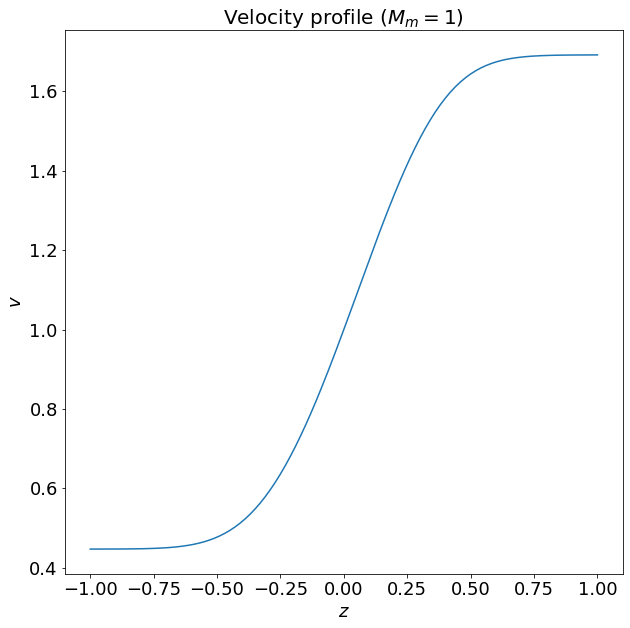
\includegraphics[width=\linewidth]{img/velocity-profile-accelerating.png}
        \caption{Accelerating velocity profile.}
    \end{subfigure}%
    \begin{subfigure}[b]{0.5\linewidth}
        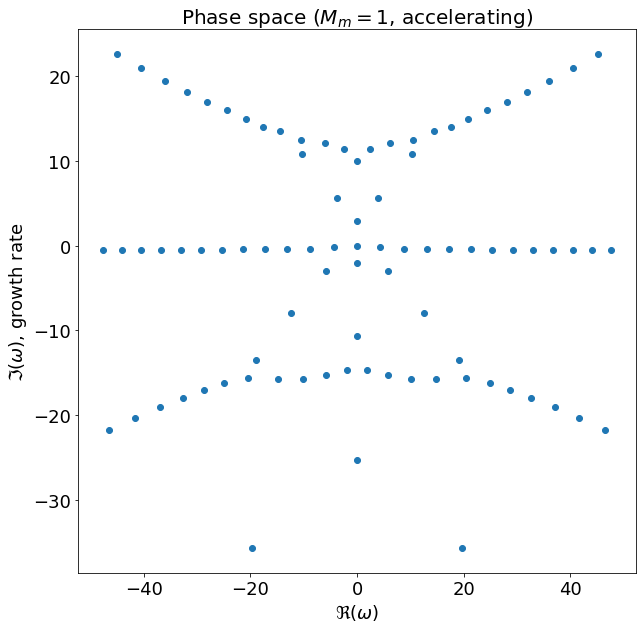
\includegraphics[width=\linewidth]{img/phase-space-accelerating.png}
        \caption{Some modes are unstable.}
    \end{subfigure}
    \caption{Solution to the polynomial eigenvalue problem Eq.(\ref{eq:polynomial-eigenvalue-problem}) with accelerating velocity profile. $\omega$'s are not on the real line, meaning that accelerating mode should be unstable for most cases.}
    \label{fig:accelerating}
\end{figure}


\newpage
\subsection{Decelerating case}
Decelerating modes are unstable.

The stability condition for ground state is $D=0.00062>0$.

\begin{figure}[H]
    \centering
    \begin{subfigure}[b]{0.5\linewidth}
        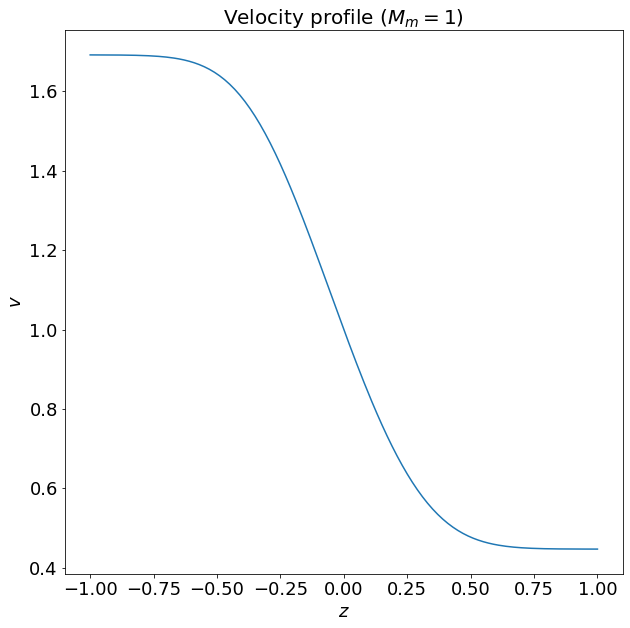
\includegraphics[width=\linewidth]{img/velocity-profile-decelerating.png}
        \caption{Decelerating velocity profile.}
    \end{subfigure}%
    \begin{subfigure}[b]{0.5\linewidth}
        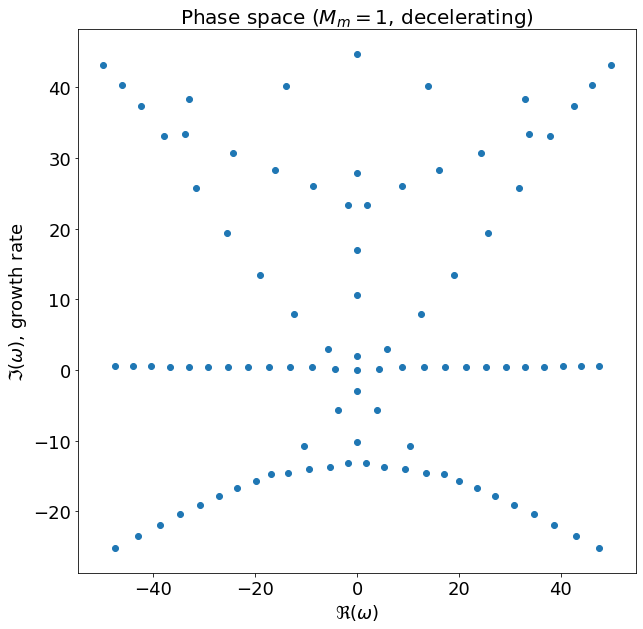
\includegraphics[width=\linewidth]{img/phase-space-decelerating.png}
        \caption{Some modes are unstable.}
    \end{subfigure}
    \caption{Solution to the polynomial eigenvalue problem Eq.(\ref{eq:polynomial-eigenvalue-problem}) with decelerating velocity profile. $\omega$'s are not on the real line, meaning that decelerating mode should be unstable for most cases.}
    \label{fig:decelerating}
\end{figure}

\newpage
\subsection{Supersonic case}
Supersonic modes are unstable.

The stability condition for ground state is $D=1.21025>0$.

\begin{figure}[H]
    \centering
    \begin{subfigure}[b]{0.5\linewidth}
        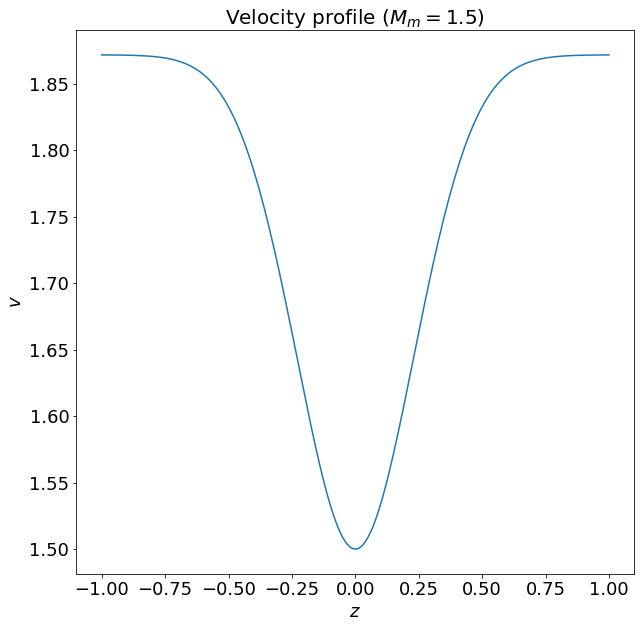
\includegraphics[width=\linewidth]{img/velocity-profile-supersonic.png}
        \caption{Supersonic velocity profile.}
    \end{subfigure}%
    \begin{subfigure}[b]{0.5\linewidth}
        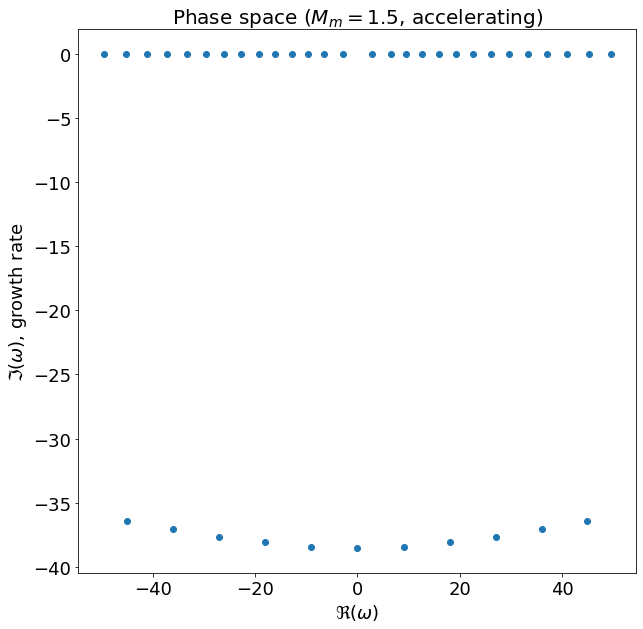
\includegraphics[width=\linewidth]{img/phase-space-supersonic.png}
        \caption{Some modes are unstable.}
    \end{subfigure}
    \caption{Solution to the polynomial eigenvalue problem Eq.(\ref{eq:polynomial-eigenvalue-problem}) with supersonic velocity profile. $\omega$'s are not on the real line, meaning that supersonic mode should be unstable for most cases.}
    \label{fig:supersonic}
\end{figure}



\end{document}


